\section{\lang{Summary of the proposed solution}{Resumen de la solución propuesta}}

\ifthenelse{\equal{\LANG}{es}}{
    Para poder aceptar o rechazar las hipótesis planteadas en la sección \ref{sec:objetivos}, se han entrenado distintos modelos con diferentes valores de un conjunto de hiperparámetros. La lista de hiperparámetros y el número de posibles valores de cada uno se puede ver en la tabla \ref{tab:hyperparameters}.
}{}
\ifthenelse{\equal{\LANG}{en}}{
    To accept or reject the hypotheses stated in Section \ref{sec:objetivos}, different models were trained with different values of a set of hyperparameters. The list of hyperparameters and the number of possible values for each one can be seen in Table \ref{tab:hyperparameters}.
}{}

\begin{table}[h]
    \centering
    {\small
        \begin{tabular}{llcr}
            \toprule
            \multirow{2}{*}{\lang{Hyperparameter}{Hiperparámetro}}                             & \multirow{2}{*}{\lang{Meaning}{Significado}}                                                                                   & \multirow{2}{*}{\lang{Appendix}{Anexo}} & \lang{Search}{Espacio}          \\
                                                                                               &                                                                                                                                &                                         & $\;\;$\lang{space}{de búsqueda} \\
            \midrule
            nTeams                                                                             & \lang{Number of teams seen.}{Número de equipos vistos.}                                                                        &                                         & 5                               \\
            nEpisodes                                                                          & \lang{Number of battles against each opponent per epoch.}{Número de batallas contra cada oponente por epoch.}                  &                                         & 5                               \\
            actor                                                                              & \lang{Actor neural-network architecture.}{Arquitectura de la red neuronal del actor.}                                          & \ref{anexo:hyperActor}                  & 4                               \\
            critic                                                                             & \lang{Critic neural-network architecture (or whether it is used).}{Arquitectura de la red neuronal del crítico (o si se usa).} & \ref{anexo:hyperCritic}                 & 5                               \\
            gamma                                                                              & \lang{Discount factor.}{Factor de descuento.}                                                                                  &                                         & 2                               \\
            reward                                                                             & \lang{Function that determines the reward for each action.}{Función que determina la recompensa de cada acción.}               & \ref{anexo:hyperReward}                 & 2                               \\
            player                                                                             & \lang{Common-field representation.}{Representación del campo en común.}                                                        & \ref{anexo:hyperPlayer}                 & 2                               \\
            pokemon                                                                            & \lang{Representation of each Pokémon.}{Representación de cada Pokémon.}                                                        & \ref{anexo:hyperPokemon}                & 12                              \\
            move                                                                               & \lang{Representation of each move.}{Representación de cada movimiento.}                                                        & \ref{anexo:hyperMove}                   & 11                              \\
            useRandom                                                                          & \lang{Train against the random opponent.}{Entrenarse contra el oponente aleatorio.}                                            &                                         & 2                               \\
            useMaxDamage                                                                       & \lang{Train against the maximum-damage opponent.}{Entrenarse contra el oponente de máximo daño.}                               &                                         & 2                               \\
            useSelfPlay                                                                        & \lang{Train against itself.}{Entrenarse contra uno mismo.}                                                                     &                                         & 2                               \\
            \midrule
            \multicolumn{3}{l}{\lang{Total number of combinations}{Nº total de combinaciones}} & 3.520.000                                                                                                                                                                                                  \\
            \bottomrule
        \end{tabular}
    }
    \caption[\lang{Set of hyperparameters with the number of possible values for each one}{Conjunto de hiperparámetros con el número de posibles valores para cada uno}]{\lang{Set of hyperparameters with the number of possible values for each one. The ``Appendix'' column indicates where more information about some of the hyperparameters can be found}{Conjunto de hiperparámetros con el número de posibles valores para cada uno. La columna ``Anexo'' indica en qué anexo se puede encontrar más información sobre algunos de los hiperparámetros}}
    \label{tab:hyperparameters}
\end{table}

\begin{description}
    \item[\HOne]
          \ifthenelse{\equal{\LANG}{es}}{
              Para evaluar la hipótesis \HOne~se han usado los hiperparámetros de \emph{player} (anexo \ref{anexo:hyperPlayer}), \emph{pokemon} (anexo \ref{anexo:hyperPokemon}) y \emph{move} (anexo \ref{anexo:hyperMove}). Estos hiperparámetros escogen las clases que se usan para representar el estado de la batalla: \emph{player} para el campo de batalla, \emph{pokemon} para cada uno de los 12 Pokémon y \emph{move} para cada uno de los 4 movimientos por Pokémon (48 movimientos en total). En base a estos hiperparámetros se configura el número de parámetros de la primera capa de la red neuronal que estará en el rango 60-82.876.
          }{}
          \ifthenelse{\equal{\LANG}{en}}{
              To evaluate hypothesis \HOne, the \emph{player} (appendix \ref{anexo:hyperPlayer}), \emph{pokemon} (appendix \ref{anexo:hyperPokemon}), and \emph{move} (appendix \ref{anexo:hyperMove}) hyperparameters were used. These hyperparameters choose the classes used to represent the battle state: \emph{player} for the battle field, \emph{pokemon} for each of the 12 Pokémon, and \emph{move} for each of the 4 moves per Pokémon (48 moves in total). Based on these hyperparameters, the number of parameters in the first neural-network layer is set from 60 to 82,876 neurons.
          }{}

    \item[\HTwo]
          \ifthenelse{\equal{\LANG}{es}}{
              Para evaluar la hipótesis \HTwo~se ha usado el hiperparámetro \emph{useSelfPlay}, que determina si el agente se entrena contra sí mismo o no. Durante el entrenamiento, se guardan los modelos correspondientes a los últimos 20 epochs y se juegan \emph{nEpisodes} partidas en total contra modelos elegidos aleatoriamente entre este conjunto de 20. También están relacionados con esta hipótesis los hiperparámetros \emph{useRandom} y \emph{useMaxDamage}, que determinan si el agente se entrena contra un oponente aleatorio o un oponente que siempre elige el movimiento que hace más daño. Es necesario que al menos uno de estos tres hiperparámetros esté activo para que el agente tenga un oponente contra el que entrenar (ver figura \ref{fig:training}).
          }{}
          \ifthenelse{\equal{\LANG}{en}}{
              To evaluate hypothesis \HTwo, the \emph{useSelfPlay} hyperparameter was used; it determines whether the agent trains against itself or not. During training, the models corresponding to the last 20 epochs are stored, and \emph{nEpisodes} games are played in total against models chosen at random from this set of 20. Also related to this hypothesis are the \emph{useRandom} and \emph{useMaxDamage} hyperparameters, which determine whether the agent trains against a random opponent or an opponent that always chooses the move that deals the most damage. At least one of these three hyperparameters must be active for the agent to have an opponent to train against (see Figure \ref{fig:training}).
          }{}

          \begin{figure}[h]
              \centering
              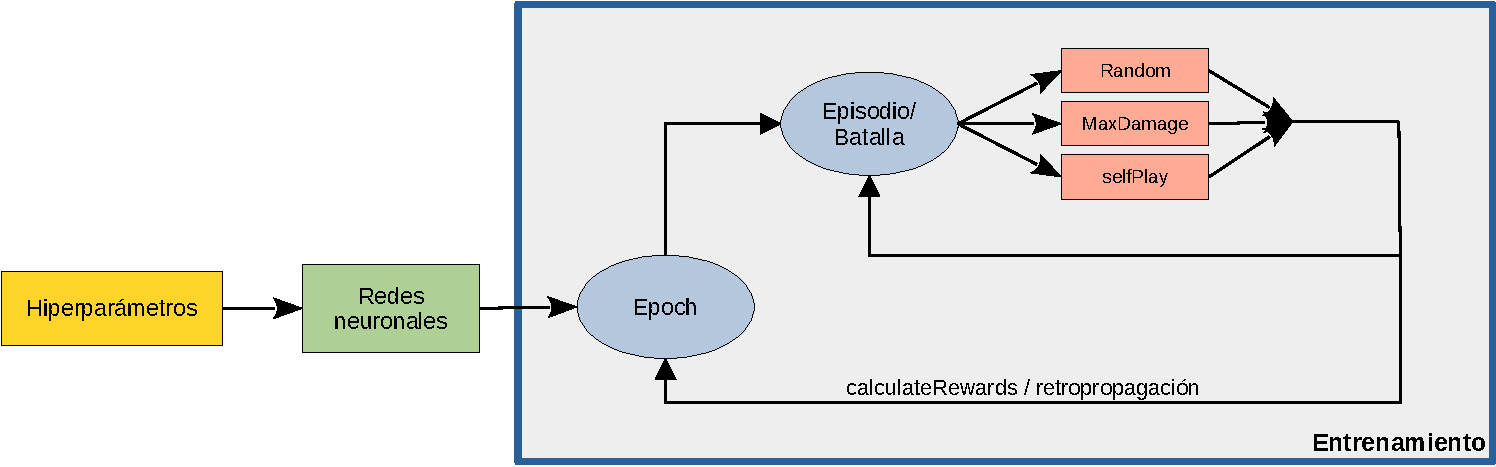
\includegraphics[width=0.9\textwidth]{images/training-crop.pdf}
              \caption{\lang{Training of an experiment}{Entrenamiento de un experimento}}
              \label{fig:training}
          \end{figure}

    \item[\HThree]
          \ifthenelse{\equal{\LANG}{es}}{
              Para evaluar la hipótesis \HThree~ se ha usado el hiperparámetro \emph{nTeams}, que determina el número de equipos que es usado para entrenar un modelo, tanto para el modelo como para el oponente. Se han probado 5 valores distintos: 1, 2, 10, 100 y inf. Para los valores finitos, los equipos son creados a priori. Para el valor infinito, se usa el formato \emph{gen9randombattle}, en el que el equipo se genera aleatoriamente en cada partida.
          }{}
          \ifthenelse{\equal{\LANG}{en}}{
              To evaluate hypothesis \HThree, the \emph{nTeams} hyperparameter was used. It determines the number of teams used to train a model, both for the model itself and for the opponent. Five different values were tested: 1, 2, 10, 100, and inf. For finite values, the teams are created a priori. For the infinite value, the \emph{gen9randombattle} format is used, in which the team is generated randomly in each match.
          }{}
\end{description}

\ifthenelse{\equal{\LANG}{es}}{
    En la tabla \ref{tab:hyperparameters} se incluyen otros hiperparámetros para poder probar la variabilidad de los resultados en relación con los hiperparámetros relativos a las hipótesis. Entre estos se incluyen el tamaño de la red (\emph{actor} y \emph{critic}), si usar critic o no (\emph{critic} vacío), el número de episodios por epoch (\emph{nEpisodes}), el factor de descuento (\emph{gamma}) y la función de recompensa (\emph{reward}).
}{}
\ifthenelse{\equal{\LANG}{en}}{
    Table \ref{tab:hyperparameters} includes other hyperparameters in order to test the variability of the results relative to the hyperparameters tied to the hypotheses. These include the network size (\emph{actor} and \emph{critic}), whether to use a critic or not (empty \emph{critic}), the number of episodes per epoch (\emph{nEpisodes}), the discount factor (\emph{gamma}), and the reward function (\emph{reward}).
}{}

\ifthenelse{\equal{\LANG}{es}}{La figura \ref{fig:general} muestra el proceso de evaluación de los hiperparámetros.}{}
\ifthenelse{\equal{\LANG}{en}}{Figure \ref{fig:general} shows the hyperparameter evaluation process.}{}

\begin{figure}[h]
    \centering
    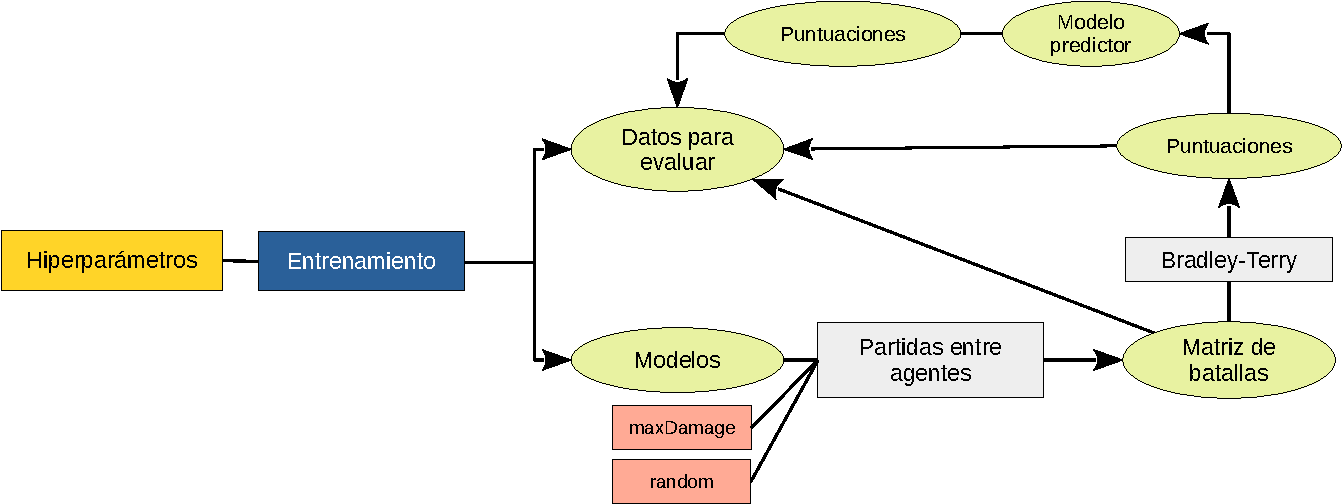
\includegraphics[width=\textwidth]{images/general-crop.pdf}
    \caption{\lang{General diagram of the project}{Diagrama general del proyecto}}
    \label{fig:general}
\end{figure}

\ifthenelse{\equal{\LANG}{es}}{
    Como probar el número total de combinaciones posibles (3.520.000) es inabordable, se han probado un subconjunto de 151 combinaciones de hiperparámetros. Cada una se entrena con una única semilla y el entrenamiento dura 1000 epochs. Una vez que ha finalizado el entrenamiento los modelos se almacenan para poder usarlos en tareas de validación. Podemos dividir las métricas obtenidas en dos tipos: las obtenidas durante el entrenamiento y las obtenidas después del entrenamiento.
}{}
\ifthenelse{\equal{\LANG}{en}}{
    Since testing the full number of possible combinations (3,520,000) is unfeasible, a subset of 151 hyperparameter combinations was tested. Each one is trained with a single seed and the training lasts 1000 epochs. Once training has finished, the models are stored so they can be used in validation tasks. The metrics obtained can be divided into two types: those obtained during training and those obtained after training.
}{}

\ifthenelse{\equal{\LANG}{es}}{Durante el entrenamiento se obtienen las siguientes métricas en cada epoch:}{}
\ifthenelse{\equal{\LANG}{en}}{During training, the following metrics are obtained in each epoch:}{}

\begin{itemize}
    \item \lang{Agent win rate across all episodes played in that epoch. High values for this parameter do not mean that an agent is stronger, since it may have been trained against weak opponents.}{Proporción de victorias del agente de todos los episodios jugados en ese epoch. Valores altos de este parámetro no significan que un agente sea más fuerte, ya que puede haber sido entrenado contra oponentes débiles.}
    \item \lang{Average actor loss normalized by the number of turns in that epoch.}{Pérdida media del actor normalizada por el número de turnos en ese epoch.}
    \item \lang{Average agent reward normalized by the number of turns in that epoch.}{Recompensa media del agente normalizada por el número de turnos en ese epoch.}
    \item \lang{Average number of turns in the battles played in that epoch.}{Número medio de turnos de las batallas jugadas en ese epoch.}
    \item \lang{If a critic is used, the average critic loss normalized by the number of turns in that epoch.}{Si se usa crítico, la pérdida media del crítico normalizada por el número de turnos en ese epoch.}
    \item \lang{If a critic is used, the average critic reward normalized by the number of turns in that epoch.}{Si se usa crítico, la recompensa media del crítico normalizada por el número de turnos en ese epoch.}
\end{itemize}

\ifthenelse{\equal{\LANG}{es}}{El resto de esta sección se refiere a las métricas obtenidas después del entrenamiento.}{}
\ifthenelse{\equal{\LANG}{en}}{The rest of this section refers to the metrics obtained after training.}{}

\ifthenelse{\equal{\LANG}{es}}{
    Como disponemos de los modelos, se pueden jugar partidas entre modelos para obtener una matriz de victorias. Por motivos de tamaño, la imagen generada con esta matriz no puede ser incluida en este documento, por lo que está disponible online\footnote{Proporción de victorias: \url{https://drive.google.com/file/d/1FIfLRBHuJ33bC_FBJho3Hk0I-aJ2glsp/view?usp=sharing}}. Cada fila representa la proporción de victorias contra el modelo de la columna. Al seguir el mismo orden de filas y de columnas, dos casillas opuestas suman 1. En cuanto a la diagonal, cada modelo compite contra él mismo por lo que la proporción de victorias es cercana a 0.5.
}{}
\ifthenelse{\equal{\LANG}{en}}{
    Since the models are available, matches can be played between models to obtain a win matrix. Because of its size, the image generated from this matrix cannot be included in this document, so it is available online\footnote{Win rate: \url{https://drive.google.com/file/d/1FIfLRBHuJ33bC_FBJho3Hk0I-aJ2glsp/view?usp=sharing}}. Each row represents the win rate against the model in the column. Because rows and columns follow the same order, two opposite cells sum to 1. As for the diagonal, each model competes against itself, so the win rate is close to 0.5.
}{}

\ifthenelse{\equal{\LANG}{es}}{
    Esta matriz incluye las victorias de: (i) los 151 modelos correspondientes a las 151 combinaciones de hiperparámetros que se han probado, (ii) el jugador aleatorio, y (iii) el jugador que siempre elige el movimiento que hace más daño. Estos dos últimos jugadores se incluyen como referencia. Inicialmente cada celda se cubre con los resultados de 10 partidas, pero posteriormente se juegan más partidas para las casillas que tienen más incertidumbre. Dicha incertidumbre se estima mediante el intervalo de Wilson~\cite{wilson1927} con un 95\% de confianza, utilizando la amplitud del intervalo (diferencia entre el límite superior y el inferior). En total se han jugado $3.711.670$ partidas. Los valores de incertidumbre también se puede consultar online\footnote{Incertidumbre: \url{https://drive.google.com/file/d/1eJBiV4Dtwemnvf0MvkRXA4L6FiXguRy6/view?usp=sharing}}.
}{}
\ifthenelse{\equal{\LANG}{en}}{
    This matrix includes the wins of: (i) the 151 models corresponding to the 151 hyperparameter combinations that were tested, (ii) the random player, and (iii) the player that always chooses the move that deals the most damage. These last two players are included as baselines. Initially, each cell is covered with the results of 10 games, but more games are later played for the cells with greater uncertainty. That uncertainty is estimated using the Wilson interval~\cite{wilson1927} with 95\% confidence, using the interval width (difference between the upper and lower bounds). In total, $3.711.670$ games were played. The uncertainty values can also be consulted online\footnote{Uncertainty: \url{https://drive.google.com/file/d/1eJBiV4Dtwemnvf0MvkRXA4L6FiXguRy6/view?usp=sharing}}.
}{}

\ifthenelse{\equal{\LANG}{es}}{
    Con la matriz de victorias, ya se puede intentar aislar los efectos de cambiar un solo hiperparámetro. Para ello se hace una matriz de victorias para cada hiperparámetro, en la que cada celda representa la media de la proporción de victorias del hiperparámetro de la fila contra el hiperparámetro de la columna. La diagonal está vacía y las casillas opuestas suman 0 porque las derrotas se contabilizan como victorias de signo negativo. Un ejemplo de una de estas matrices se puede ver en la figura \ref{fig:battlesMove} (página~\pageref{fig:battlesMove}).
}{}
\ifthenelse{\equal{\LANG}{en}}{
    With the win matrix, it is then possible to try to isolate the effects of changing a single hyperparameter. To do this, a win matrix is built for each hyperparameter, in which each cell represents the mean win rate of the row hyperparameter against the column hyperparameter. The diagonal is empty and opposite cells sum to 0 because losses are counted as negative wins. An example of one of these matrices can be seen in Figure \ref{fig:battlesMove} (page~\pageref{fig:battlesMove}).
}{}

\ifthenelse{\equal{\LANG}{es}}{
    Una vez que se tiene la matriz de victorias, se puede aplicar un modelo Bradley-Terry~\cite{bradleyterry1952} para calcular una puntuación de fuerza para cada modelo. Esto ha sido implementado manualmente usando un modelo de regresión logística. Con esto podemos ver que el modelo que siempre elige el movimiento de máximo daño está apreciablemente por encima de los demás y que el jugador aleatorio es un jugador en una posición intermedia de la tabla. La tabla completa está disponible en el Anexo~\ref{anexo:bradleyterry} (página~\pageref{anexo:bradleyterry}).
}{}
\ifthenelse{\equal{\LANG}{en}}{
    Once the win matrix is available, a Bradley-Terry model~\cite{bradleyterry1952} can be applied to compute a strength score for each model. This has been implemented manually using a logistic regression model. This shows that the model that always chooses the maximum-damage move is appreciably above the others, and that the random player sits in the middle of the table. The full table is available in Appendix~\ref{anexo:bradleyterry} (page~\pageref{anexo:bradleyterry}).
}{}

\ifthenelse{\equal{\LANG}{es}}{
    Una vez obtenidas las puntuaciones de Bradley-Terry, se puede intentar predecir la puntuación de fuerza de un modelo a partir de sus hiperparámetros. Para ello se ha entrenado un modelo \emph{GradientBoostingRegressor} de la librería \emph{scikit-learn} que a partir de ahora será llamado modelo predictor (\textit{surrogate model}). Este modelo predictor es capaz de estimar la fuerza de un modelo a partir de los valores de sus hiperparámetros, lo que es útil para entrenar de manera óptima nuevos modelos.
}{}
\ifthenelse{\equal{\LANG}{en}}{
    Once the Bradley-Terry scores have been obtained, it is possible to try to predict a model's strength score from its hyperparameters. To do this, a \emph{GradientBoostingRegressor} model from the \emph{scikit-learn} library was trained and will hereafter be called the surrogate model (\textit{surrogate model}). This predictor model is capable of estimating a model's strength from the values of its hyperparameters, which is useful for training new models optimally.
}{}

\ifthenelse{\equal{\LANG}{es}}{
    Usando el modelo predictor, también es posible intentar aislar un hiperparámetro y estudiar la influencia de dicho hiperparámetro en la fuerza de los modelos. Se pueden generar matrices cuadradas iguales a las de victorias, pero debido a que se usa un modelo predictor entrenado con solo $151$ datos de entrenamiento, su funcionalidad resulta limitada. Por ejemplo, en el caso del hiperparámetro \emph{nTeams} el modelo predictor da una matriz completamente opuesta a la de victorias.
}{}
\ifthenelse{\equal{\LANG}{en}}{
    Using the surrogate model, it is also possible to try to isolate a hyperparameter and study that hyperparameter's influence on model strength. Square matrices like the win matrices can be generated, but because a surrogate model trained with only $151$ training data points is used, its functionality is limited. For example, in the case of the \emph{nTeams} hyperparameter, the surrogate model produces a matrix completely opposite to the win matrix.
}{}
